\lettrine[lines=2,findent=2pt,nindent=3pt,loversize=0.1]{\textcolor[gray]{0.4}{L}}{a} industria del videojuego en España, sigue siendo líder en el ocio audiovisual \cite{1}, con casi 16 millones de jugadores. La facturación de esta industria, supera a la suma conjunta de las facturaciones del cine y la música. Los datos del 2017 indican un crecimiento del $16.9$\% con respecto al año 2016, por lo que se puede observar que la industria del videojuego sigue en aumento. Aunque la industria del videojuego en España aun no es un motor de crecimiento, tiene un importante impacto económico \cite{2}, generando alrededor de 8000 empleos directos, cada uno de los cuales genera a su vez $2.6$ empleos indirectos.

Los datos también revelan que la población española tiende a consumir videojuegos ya que aproximadamente un 44\% de los españoles entre 6 y 64 años juega a videojuegos. Esto significa que en España existen $15.8$ millones de jugadores. De entre los españoles que juegan a videojuegos, un 44\% son mujeres. La franja de edad con más jugadores va desde los 15 hasta los 44 años. El tiempo medio que la población española le dedica a jugar videojuegos es de $6,6$ horas, un consumo aceptable con respecto a otros países europeos.

En los últimos años la popularidad de los videojuegos ha aumentado en parte gracias a los \textbf{eSports}. España es el octavo país en el ránking de audiencia de eSports. Debido a la popularidad de los mismos en el país, se generan 300 puestos de empleo y hay unos 100 jugadores profesionales de eSports.

Según la \acf{DEV} \cite{3}, en el año 2016 había un total de 5440 profesionales trabajando en la industria del videojuego en España. Las previsiones de crecimiento de este dato son del $20,37$\% anual, hasta llegar a unos 11420 empleos directos en el año 2020. Los datos de empleo de desarrolladores de videojuego son claros: aproximadamente un 62\% de las empresas en España tienen problemas para encontrar especialistas en programación de videojuegos. 

Aunque España es uno de los países con más jugadores de videojuegos, existen pocos estudios de desarrollo que superen las 30 personas \cite{4}. La mayoría de los estudios que existen en el país están formados por menos de 5 personas y de cada 10 proyectos que se lanzan, unos 8 cierran por motivos principalmente comerciales. Es difícil dar a conocer tu producto en esta industria. Además estos estudios están formados principalmente por diseñadores y desarrolladores, por lo que la experiencia en \textit{marketing} es baja.

Antiguamente, cada compañía que realizaba un videojuego, empleaba la mayor parte del desarrollo del mismo en crear un motor de videojuegos desde cero, que lo utilizarían para llevar a cabo el proyecto. La reutilización de los motores era generalmente pobre, de forma que se usaba un motor nuevo (o prácticamente nuevo) por cada videojuego desarrollado. Esto hacía que cada desarrollo fuese muy prolongado en duración, los costes del proyecto subían y por tanto, los riesgos de pérdidas eran también mayores. También existe la falsa creencia de que si no desarrollas por completo el motor gráfico, no eres realmente un programador de videojuegos. Esta creencia está desapareciendo con los años, ya que no es sencillo que una empresa independiente que desarrolla videojuegos consiga suficientes ganancias de su desarrollo, por lo que un sobrecoste como puede ser el motor gráfico puede hacer que el desarrollo tenga que abortarse.

\pagestyle{notsection}

Hoy en día, la mayoría de las empresas usan un motor gráfico comercial como puede ser Unreal Engine\footnote{https://www.unrealengine.com} o Unity\footnote{https://unity3d.com}, entre otros. Algunos de estos motores gráficos son de uso gratuito y tan sólo debes pagar a la empresa que lo desarrolla si al publicar el videojuego, supera un umbral de ganancias. Sin embargo, otros de ellos conllevan una licencia de uso que lleva asociada consigo un coste específico. Con el paso de los años, los motores gráficos son cada vez más potentes y más versátiles, por lo que se adaptan a muchos tipos de videojuegos y el rendimiento que ofrecen es muy bueno. Debido a esto, se han convertido en una opción a tener muy en cuenta cuando se quiere desarrollar un videojuego. 

Un motor gráfico \cite{5} es un software que está diseñado para crear y desarrollar videojuegos. Se pueden desarrollar videojuegos para consolas, dispositivos móviles, ordenadores o dispositivos de \acf{RV}. Los motores gráficos separan los componentes de renderizado gráfico, de audio, de colisiones, multijugador, de inteligencia artificial, etc. para permitir una mayor reutilización en varios juegos.

Unreal Engine es un motor de videojuegos que nació en el año 1998, desarrollado por la compañía Epic Games\footnote{\url{https://www.epicgames.com/site}}. La versión del motor a día de hoy es \acf{UE4}, sucesor del \textit{\acf{UDK}}. Este motor esta orientado principalmente a los \textit{shooters} en primera persona (\acf{FPS}), aunque \acs{UE4} es tan potente que se puede desarrollar cualquier tipo de videojuego.

\begin{figure}[h]
\centering
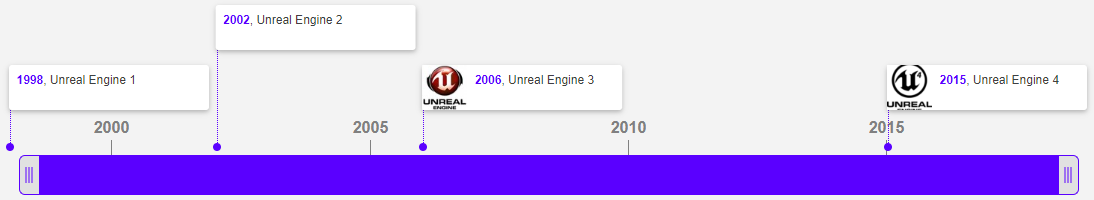
\includegraphics[width=15cm]{./images/timeline.png}
\caption{Timeline de Unreal Engine}
\end{figure}

\acs{UE4} permite portar los videojuegos a distintas plataformas, como son: PC, PlayStation 4, Xbox One, Android, iOS y Mac. Además, posee un gran soporte para dispositivos de \ac{RV}. Por esto, \acs{UE4} es uno de los motores más populares entre los desarrolladores de videojuegos. 

\acs{UE4} posee un lenguaje de \textit{scripting} visual, denominado \textit{Blueprints}. Es un método de \textit{scripting} basado en nodos haciendo que no se necesite escribir ni una sola línea de código. Este método es muy usado para realizar prototipados rápidos de niveles. En un desarrollo completo de un videojuego, se combina la facilidad de uso de \textit{Blueprints} con la potencia del lenguaje de programación C++. Dicho lenguaje, es el lenguaje de facto en la industria de los videojuegos ya que ofrece un gran rendimiento (algo esencial en cualquier videojuego) y las posibilidades con C++ quedan limitadas tan solo por el programador.

El acceso al código fuente\footnote{https://github.com/EpicGames/UnrealEngine} completo del motor de \acs{UE4} aumenta aun más las posibilidades que ofrece \cite{6}. Se puede modificar el código fuente para aumentar el rendimiento de un desarrollo en específico, se pueden introducir nuevas características al motor que no estén ofrecidas de forma oficial por Epic Games pero que sean necesarias para un desarrollo puntual. En este contexto surgen los \textit{plugins}, como un medio para lograr explotar mejor el uso del motor de videojuegos. \acs{UE4} posee un \textit{marketplace}\footnote{https://www.unrealengine.com/marketplace/store} en el que se pueden encontrar muchos \textit{plugins} tanto gratuitos como de pago. El código fuente del motor es también útil en labores de depuración del videojuego, para entender mejor las interacciones entre el código del videojuego y el código del motor.

\acs{UE4} posee muchas características que hacen que sea uno de los motores gráficos más potentes hoy en día. Posee un editor para personalizar los sistemas de partículas, una potente solución para desarrollos de \ac{RV}, un gran editor de materiales, lo que permite crear texturas en el propio motor, sin necesidad de acudir a programas de terceros. El módulo de \ac{IA} es muy potente y fácil de usar. Se pueden crear paisajes de una forma rápida y sencilla con el módulo de Terreno y Follaje. Este módulo permite crear entornos de mundo abierto gracias al uso eficiente de la memoria y al sistema \ac{LOD} que ajusta la complejidad de los objetos en función de la distancia, para priorizar el rendimiento. Las características de post-procesado en \acs{UE4}, aumentan la calidad de los resultados visuales finales en las escenas.

Los juegos multijugador \cite{7} son uno de los mercados más buscados por los jugadores de videojuegos, principalmente por la capacidad de diversión que ofrecen los mismos, al poder interactuar con otros jugadores. En un principio, los humanos tienen una capacidad de estrategia mayor que la máquina y una inteligencia artificial muy potente requiere de una gran capacidad de cómputo. El ser humano es un ser social por naturaleza, por lo que los videojuegos multijugador tienden a ser más atractivos para la mayoría de la población.

En los juegos de multijugador local, dos o más jugadores juegan en un mismo computador, por lo que el desarrollo del videojuego es prácticamente idéntico, con las únicas diferencias de un mayor soporte a dispositivos de entrada/salida y distintos puntos de vista para los distintos jugadores. En los juegos multijugador en \ac{LAN} se encuentran varias computadoras conectadas unas con otras a través de una misma red. Este es realmente el modelo más básico de videojuegos multijugador.

En los videojuegos online, los jugadores se conectan con otros a través de grandes redes, dónde los computadores se pueden encontrar geográficamente muy distantes los unos con los otros. Tradicionalmente, se usan arquitecturas basadas en el modelo cliente-servidor \cite{8} durante el desarrollo de un videojuego online debido a que es más sencillo securizar e implementar esta solución. La partida se lleva a cabo en el servidor y los clientes simplemente renderizan la partida con los datos que reciben del servidor y recogen los eventos de entrada. Hoy en día la mayoría de juegos online permiten un número relativamente pequeño de conexiones simultáneas por sesión (de 4 a 32, normalmente). Sin embargo existen los juegos de tipo multijugador masivo o \ac{MMG}, en los que cientos o miles de jugadores pueden participar en una misma sesión.

La mayor cuestión a tener en cuenta en los videojuegos online es la latencia, entendida como la cantidad de tiempo que tardan los datos del videojuego en viajar por la red. Las \ac{LAN} proporcionan características como \textit{broadcast}, una baja latencia, un gran ancho de banda y apenas pérdida de paquetes. La calidad de las conexiones de red sobre internet son muy difíciles de predecir ya que no es factible crear conexiones punto a punto para muchos clientes. Los principales problemas en videojuegos online \cite{9} son la latencia, el \textit{jitter} y un ancho de banda bajo. Puesto que el \textit{multicast} no es soportado por todos los protocolos, el ancho de banda se ve perjudicado al tener que enviar el mismo paquete una vez (como mínimo) a cada cliente conectado. Los mecanismos de predicción pueden hacer que la experiencia de juego con una latencia alta mejore, sin embargo un \textit{jitter} alto hace que el juego sea prácticamente injugable.

Desarrollar un juego multijugador online no es una tarea sencilla, ya que es uno de los tipos de juegos más difíciles de desarrollar. Hay que tener en cuenta todas estas cuestiones anteriores y muchas otras, como la relevancia de los datos (puede que ciertas zonas del mapa que no son accesibles no tengan necesidad de intercambiar información. Teniendo esta cuestión en mente, se puede disminuir considerablemente el ancho de banda usado), además de necesitar un alto conocimiento en redes y sistemas distribuidos. Sin embargo \acs{UE4} proporciona un módulo multijugador\footnote{\url{https://www.unrealengine.com/en-US/blog/getting-started-with-unreal-multiplayer-in-cpp}} que facilita mucho la tarea de desarrollar un juego online. Si dicho módulo se combina con el \ac{SDK} o Kit de Desarrollo de Software de STEAM\footnote{\url{https://wiki.unrealengine.com/Steam,_Using_the_Steam_SDK_During_Development}} se pueden crear, buscar y unirse a sesiones de una forma sencilla.

\acs{UE4} también hace esfuerzos por mejorar la experiencia de usuario cuando existe una latencia alta. Implementa técnicas sobre el componente de movimiento de los personajes que hace que el jugador no note esa alta latencia cuando se está moviendo, en un juego de tipo \acs{FPS}).

Según \cite{10}, un videojuego debe proporcionar al jugador retos de una dificultad intermedia. Los elementos que determinan el nivel de motivación del desafío son:

\begin{itemize}
\item Los objetivos.
\item La incertidumbre del resultado.
\item La retroalimentación del desempeño.
\end{itemize}

Para que un reto sea motivante, las metas deben estar claramente definidas y organizadas en una jerarquía que relacione los objetivos a corto y a largo plazo. El resultado del juego debe ser incierto, usando niveles de dificultad variable, distintos niveles de metas, información oculta y aleatoriedad, para evitar la trivialidad y las dificultades casi imposibles. Para mantener la motivación, la retroalimentación debe ser clara, constructiva y alentadora, lo que contribuirá a la autoestima del jugador.

Sobre esta definición encajan perfectamente los videojuegos de acción, con una campaña motivada por una historia profunda, que acompañada de una dificultad acorde al jugador hacen que la experiencia de usuario sea motivante y adictiva de jugar. En este contexto nace este proyecto, un videojuego de acción en tercera persona, con una campaña cooperativa con la posibilidad de que dos jugadores de forma online la completen. Como aliciente en la motivación del usuario, se ha optado por introducir minijuegos para poder acceder a ciertas zonas del mapa de forma que no se pierde el contacto con la historia principal y se introduce una nueva mecánica de juego con el objetivo de entretener al jugador. 

Existen una gran variedad de modelos de negocio en la industria del videojuego, que utilizan las compañías para monetizar sus productos. Sin embargo, muchos de ellos suelen encajar dentro de otros, con pequeñas variaciones. Podríamos decir que desde una perspectiva general existen los siguientes modelos de negocio básicos:

\begin{itemize}
\item Modelo \textit{Pay-to-Play}. En este modelo, se compra el contenido del juego completo por una cierta cantidad y se pueden acceder a todas las características del mismo, sin ningún tipo de limitación. Es el modelo que más se usaba, hasta que otro tipo de modelos de negocio le han ido ganando territorio.
\item Modelo \textit{Free-to-Play}. Este modelo consiste en ofrecer el contenido del videojuego gratis. La monetización vendrá de las compras de objetos dentro del juego (como pueden ser objetos decorativos, \textit{skins} para los personajes o distintos camuflajes para las armas, entre otros) y por la publicidad existente en el juego.
\item Modelo \textit{Freemium}. Este modelo consiste en ofrecer gratis el contenido del videojuego, pero no la totalidad del mismo. Se accede a una parte del videojuego limitada y en el caso de querer acceder a más partes del mismo, tendrás que pagar una determinada cantidad de dinero. Este modelo tiene otras variantes como pagar inicialmente una cantidad y acceder a cierta funcionalidad del juego. Si quieres acceder a nuevas funcionalidades, nuevos mapas, etc., hay que comprarlo a parte.
\item Modelo de Suscripción. En este modelo, se paga el contenido por una determinada cantidad de tiempo, durante el cual se puede disfrutar del videojuego. Pasado este tiempo, la suscripción se cancela y habría que volver a pagar para jugar durante más tiempo.
\end{itemize}

En los últimos años, ha ganado mucha popularidad el contenido descargable o \ac{DLC}. Se trata de contenido digital exclusivo y adicional de un videojuego, que se vende por separado y posterior al lanzamiento del mismo. Se usan para alargar el tiempo de vida del videojuego, ofreciendo nuevos mapas, armas, personajes, etc. La obtención de los \ac{DLC} no tiene sentido si no se ha obtenido antes el videojuego, ya que son productos complementarios y dependientes del juego. En numerosas ocasiones, los \ac{DLC} están sujetos a controversia ya que se venden desde el día de lanzamiento del juego, por lo que el contenido del \ac{DLC} podría estar listo para la fecha de lanzamiento del juego y podría estar incluido dentro del mismo.

Un concepto novedoso pero que cada día está ganando más adeptos es el de \textit{game as a service} \cite{11}. Este modelo de negocio es complementario al \textit{software as a service} e implica que al ser un servicio, el usuario se beneficia durante un periodo de tiempo del mismo pero no le pertenece nada, el videojuego no es suyo nunca. Dentro del \textit{game as a service} podemos encontrar el modelo de suscripción comentado anteriormente. En muchos \ac{MMO} se usan suscripciones mensuales para poder disfrutar del videojuego.

Compañías como EA\footnote{https://www.ea.com} y Xbox\footnote{https://www.xbox.com} garantizan a sus suscriptores un acceso a una gran biblioteca de títulos que se ofrecen de forma digital sin limitación. El usuario tiene que descargar esos juegos en su ordenador o su consola para poder jugar. Sin embargo, para poder disfrutar de los juegos, el usuario debe seguir pagando la suscripción mensual.

Algunas compañías como PlayStation\footnote{https://www.playstation.com} o GameFly\footnote{https://www.gamefly.com} permiten que los usuarios jueguen los videojuegos que se ejecutan en servidores remotos en un dispositivo local, eliminando la necesidad de especialización en el hardware o la necesidad de computadores potentes para jugar. Esta forma de negocio se denomina \textit{cloud gaming}.












